\section{Auswertung}

Im Folgenden werden die erhobenen Messdaten ausgewertet, mit dem Ziel
die Landé-Faktoren der aufgespalteten roten und blauen Spektrallinie bei verschiedener
Polarisation zu bestimmen.

\subsection{Hysterese}

Der aufsteigenden Hysteresekurve wurde eine Polynomgleichung dritten Gerades zugesprochen,
welche die folgenden Einträge hat.
\begin{equation}
  \label{eqn:Hysterese_fit}
  A_1 \cdot x^3 + A_2 \cdot x^2 + A_3 \cdot x + A_4
\end{equation}
\begin{description}
  \item[$A_1$] $\SI{-0.082(7)}{\milli\tesla\per\ampere^3}$
  \item[$A_2$] $\SI{1.757(236)}{\milli\tesla\per\ampere^2}$
  \item[$A_3$] $\SI{49.121(2104)}{\milli\tesla\per\ampere}$
  \item[$A_4$] $\SI{14.152(4984)}{\milli\tesla}$
\end{description}

Für die absteigende Hysteresekurve wurde ebenfalls eine Augleichsrechnung an die
Gleichung \eqref{eqn:Hysterese_fit} betrieben.
\begin{description}
  \item[$A_1$] $\SI{-0.067(6)}{\milli\tesla\per\ampere^3}$
  \item[$A_2$] $\SI{1.217(191)}{\milli\tesla\per\ampere^2}$
  \item[$A_3$] $\SI{54.665(1703)}{\milli\tesla\per\ampere}$
  \item[$A_4$] $\SI{6.666(4033)}{\milli\tesla}$
\end{description}

Die Ausgleichsrechnungen wurden mit Hilfe des \emph{Python}-Paketes
\emph{SciPy-$curve\_fit$} durchgeführt.

Die Ausgleichsfunktionen sind im Folgenden graphisch dargestellt.

\begin{figure}
  \centering
  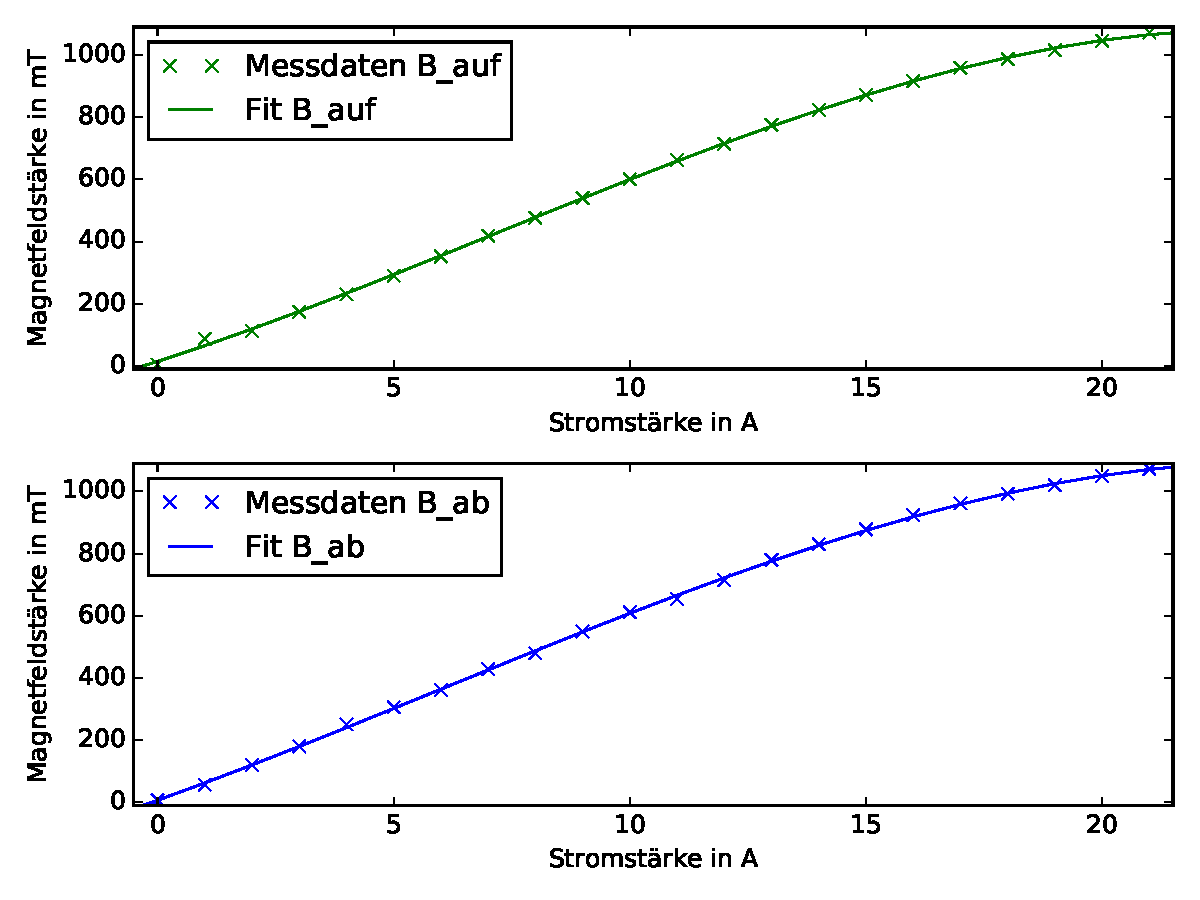
\includegraphics[width=\textwidth]{Python/Hysterese.pdf}
  \caption{Messdaten der Hysteresekurve mit eingetragenen Ausgleichsfunktionen.
  Dabei wurde die gemessene B-Feldstärke in mT gegenüber dem Strom I in A aufgetragen.}
  \label{fig:Hysterese}
\end{figure}

\begin{figure}
  \centering
  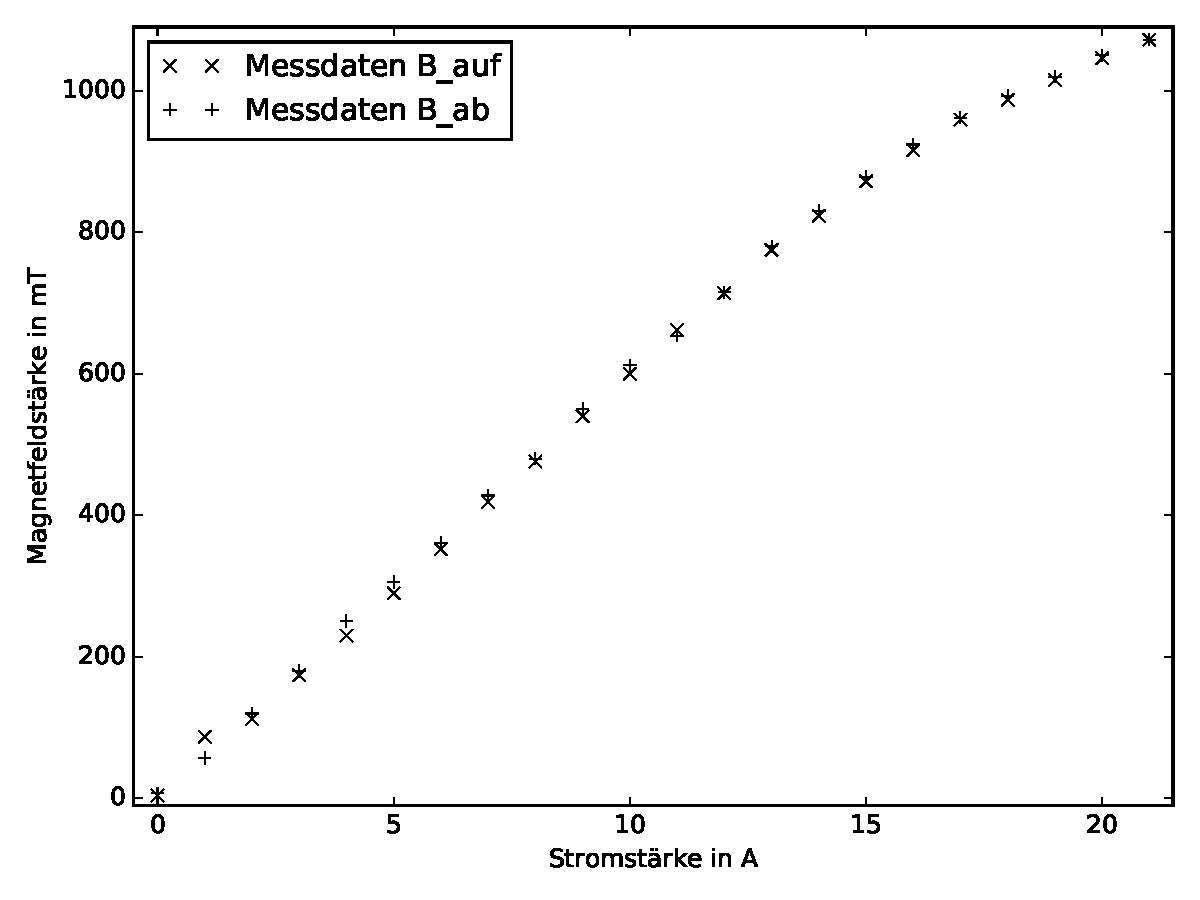
\includegraphics[width=\textwidth]{Python/Hysterese_Messdaten.pdf}
  \caption{Messdaten der gemessenen B-Feldstärke in Abhängigkeit von der Stromstärke.}
  \label{fig:Hysterese_Messdaten}
\end{figure}

Die in den Grafiken verwendeten Daten sind in Tabelle \ref{tab:Hysterese} dargestellt.

\newpage

\subsection{Vorgehensweise zur Auswertung der Spektrallinien}

Die Auswertung wird gemäß der in \cite{anleitung01} beschriebenen Vorgehensweise durchgeführt.
Prinzipiell werden die Landé-Faktoren der Spektrallinien über die Formel
\eqref{eqn:EdiffZeemanAnomal} bestimmt. Dafür werden Bilder der aufgespalteten
Linien aufgenommen, um die Distanz der Aufspaltung ($\delta S$) in Pixeln zu bestimmen.
Danach wird aus den Bildern bei $\symup{B} = \SI{0}{\milli\tesla}$ der Abstand der
unaufgespaltenen Linien $\Delta S$ in Pixeln bestimmt.
Aus diesen Daten wird die Wellenlängenveränderung $\delta\lambda$ über die Gleichung
\eqref{eqn:del_lambda} ermittelt.

\begin{equation}
  \label{eqn:del_lambda}
  \delta\lambda = \frac{1}{2}\frac{\delta S}{\Delta S}\cdot \Delta\lambda\ua{D}
\end{equation}

Dabei ist $\Delta\lambda\ua{D}$ über den Zusammenhang \eqref{eqn:DispersionsLambda}
gegeben.

Die Verschiebung in der Wellenlänge $\Delta\lambda$ entspricht
der Verschiebung in der Frequenz $\Delta\nu$, sodass der Zusammenhang
\eqref{eqn:energie_frequenz} aufgestellt werden kann.

\begin{equation}
  \label{eqn:energie_frequenz}
  \Delta E = h\cdot \Delta\nu = \frac{h\cdot c}{\delta\lambda^2}
\end{equation}

Der Landé-Faktor bestimmt sich durch die Gleichung \eqref{eqn:Landé}.

\begin{equation}
  \label{eqn:Landé}
  g = \frac{\Delta E}{\mu\ua{B} \cdot \symup{B(I)}}
\end{equation}

Dabei ist $\symup{B(I)}$ die B-Feldstärke in Abhängigkeit
von dem anliegenden Strom $\symup{I}$.

\subsection{Auswertung der roten Spektrallinie}

Von der Cadmium Spektrallampe wird die rote Spektrallinie
untersucht.
Die Kenngrößen der Lummer-Gehrcke-Platte für rotes Licht, sowie
die Wellenlänge $\lambda\ua{r}$ vom rotem Licht sind in Tabelle \ref{tab:Kenngrößen_ROT}.

\begin{table}
\centering
\caption{Kenngrößen für die rote Spektrallinie\cite{anleitung01}}
\label{tab:Kenngrößen_ROT}
\begin{tabular}{S S S }
\toprule
{Brechungsindex  $n\ua{r}$} & {Dicke $\frac{d}{\si{\milli\meter}}$} & {Wellenlänge $\frac{\lambda\ua{r}}{\si{\nano\meter}}$}  \\
\midrule
 1.4567  & 4  & 643.2\\
\bottomrule
\end{tabular}
\end{table}

In Abbildung \ref{fig:ROT_Bilder} sind die aufgenommenen Bilder der untersuchten
Interferenzmuster der roten Spektrallinie gezeigt.

\begin{figure}
  \centering
  \includegraphics[width= 8cm, height = 5cm]{Pics/ROT_zusammengefuegt.pdf}
  \caption{Untersuchte Aufnahmen der roten Spektrallinie.
  Das obere Bild wurde bei I = 0A aufgenommen. Das mittlere Bild wurde bei 9,2 A aufgenommen und zeigt die $\sigma$-Aufspaltung.
  Das untere Bild wurde ebenfalls bei I = 9,2 A aufgenommen und zeigt die $\pi$-Aufspaltung.}
  \label{fig:ROT_Bilder}
\end{figure}

\subsubsection{Sigma--Komponente der roten Spektrallinie}

Die Abstände der Intensitätsmaxima des mittleren Bildes von
Abbildung \ref{fig:ROT_Bilder} sind in Tabelle \ref{tab:rot_sigma}
dargestellt.

Mit den erhobenen Messdaten ergibt sich über \eqref{eqn:Landé}
der Landé-Faktor zu $g\ua{r,\sigma} = \num{1.14(4)}$.

\begin{table}
\centering
\caption{Messdaten der roten $\sigma$-Aufspaltung}
\label{tab:rot_sigma}
\begin{tabular}{S S}
\toprule
{$\frac{\Delta S_{\symup{r}, \sigma}}{\symup{px}}$} & {$\frac{\delta S_{\symup{r}, \sigma}}{\symup{px}}$} \\
\midrule
281.0  & 142.0\\
253.5  & 132.0\\
237.5  & 110.5\\
226.5  & 108.0\\
209.5  & 103.0\\
197.5  & 98.5\\
192.5  & 95.5\\
186.0  & 92.5\\
175.5  & 90.0\\
\bottomrule
\end{tabular}
\end{table}


\subsubsection{Pi--Komponente der roten Spektrallinie}

Die $\pi$-Komponente der roten Spektrallinie spaltet nicht auf.
Dies ist in dem unteren Bild von Abb. \ref{fig:ROT_Bilder} dargestellt.
Somit ist der Landé-Faktor gleich $g\ua{r,\pi} = \num{0}$.


\subsection{Auswertung der blauen Spektrallinie}

Methodisch gleich wie die rote Spektrallinie wird die blaue Spektrallinie
der Cadmium Lampe ausgewertet.
Die Wellenlänge und der Brechungsindex der
Lummer-Gehrcke-Platte für blaues Licht sind in Tabelle
\ref{tab:Kenngrößen_BLAU} aufgeführt.

\begin{table}
\centering
\caption{Kenngrößen für die rote Spektrallinie\cite{anleitung01}}
\label{tab:Kenngrößen_BLAU}
\begin{tabular}{S S}
\toprule
{Brechungsindex $n\ua{b}$} &  {Wellenlänge $\frac{\lambda\ua{b}}{\si{\nano\meter}}$}  \\
\midrule
 1.4635 & 480.0\\
\bottomrule
\end{tabular}
\end{table}
\FloatBarrier

\subsubsection{Sigma--Komponente der blauen Spektrallinie}

Die zur Auswertung der Aufspaltung der $\sigma$-Komponente verwendeten Bilder sind
in Abb. \ref{fig:BLAU_sigma_Bilder} dargestellt.

\begin{figure}
  \centering
  \includegraphics[width= 8cm, height = 5cm]{Pics/BLAU_zusammengefuegt_sigma.pdf}
  \caption{Untersuchte Aufnahmen der blauen Spektrallinie.
  Das obere Bild wurde bei I = 0A aufgenommen.
  Das untere Bild wurde bei 5,6 A aufgenommen und zeigt die $\sigma$-Aufspaltung.}
  \label{fig:BLAU_sigma_Bilder}
\end{figure}

Die erhobenen Messdaten zu den Intensitätsmaximaabständen
sind in Tabelle \ref{tab:blau_sigma} angegeben.
Mit den Daten aus \ref{tab:Kenngrößen_BLAU} und \ref{tab:blau_sigma}
ergibt sich der Landé-Faktor über \eqref{eqn:Landé} zu
$g\ua{b,\sigma} = \num{1.82(19)}$.

\begin{table}
\centering
\caption{Messdaten der blauen $\sigma$-Aufspaltung}
\label{tab:blau_sigma}
\begin{tabular}{S S }
\toprule
{$\frac{\Delta S_{\symup{b}, \sigma}}{\symup{px}}$} & {$\frac{\delta S_{\symup{b}, \sigma}}{\symup{px}}$} \\
\midrule
291.0  & 119.0\\
286.5  & 125.0\\
210.5  & 119.0\\
226.0  & 101.0\\
200.0  & 95.0\\
188.5  & 104.0\\
184.0  & 86.0\\
170.5  & 82.0\\
166.5  & 80.0\\
\bottomrule
\end{tabular}
\end{table}


\subsubsection{Pi--Komponente der blauen Spektrallinie}

Die ausgewerteten Bilder der Aufspaltung der $\pi$-Komponente der blauen
Spektrallinie sind in Abb. \ref{fig:BLAU_pi_Bilder} abgebildet.

\begin{figure}
  \centering
  \includegraphics[width= 8cm, height = 5cm]{Pics/BLAU_zusammengefuegt_pi.pdf}
  \caption{Untersuchte Aufnahmen der blauen Spektrallinie.
  Das obere Bild wurde bei I = 0A aufgenommen.
  Das untere Bild wurde bei 21,0 A aufgenommen und zeigt die $\pi$-Aufspaltung.}
  \label{fig:BLAU_pi_Bilder}
\end{figure}


Die erhobenen Messdaten zu den Intensitätsmaximaabständen
sind in Tabelle \ref{tab:blau_pi} dargestellt.
Mit den Daten aus \ref{tab:Kenngrößen_BLAU} und \ref{tab:blau_pi}
ergibt sich der Landé-Faktor über \eqref{eqn:Landé} zu
$g\ua{b,\sigma} = \num{0.56(4)}$.

\begin{table}[h]
\centering
\caption{Messdaten der blauen $\pi$-Aufspaltung}
\label{tab:blau_pi}
\begin{tabular}{S S}
\toprule
{$\frac{\Delta S_{\symup{b}, \pi}}{\symup{px}}$} & {$\frac{\delta S_{\symup{b}, \pi}}{\symup{px}}$} \\
\midrule
337.5  & 177.0\\
288.5  & 144.0\\
255.0  & 117.5\\
219.0  & 102.5\\
224.0  & 92.0\\
183.0  & 91.0\\
184.5  & 84.0\\
177.5  & 83.5\\
164.0  & 77.5\\
\bottomrule
\end{tabular}
\end{table}


\section{Diskussion}

Im Folgenden werden die ausgewerteten Messdaten und Ergebnisse mit den
berechneten Werten verglichen und bezüglich ihrer Aussagekraft interpretiert.
Die Ergebnisse und die berechneten Werte sind in Tab. \ref{tab:Ergebnisse} aufgeführt.
Die Fehlerintervalle der Landé-Faktoren entstehen durch die Ausgleichsrechnung für
die B-Feldstärke.
Es wurden keine Ablesefehler bei der Aufnahme des Stromes angenommen, was im
Hinblick auf den Versuch die Aussagekraft der Ergebnisse mindert.
Der gemessenen Landé-Faktor der roten $\sigma$-Komponente liegt nahezu im
Fehlerbereich und
stellt unter Berücksichtigung des vernachlässigten Ablesefehlers des Stroms
keine maßgebliche Abweichung dar.
Die gemessene $\pi$-Komponente der blauen Spektrallinie ist lediglich $\num{0,06(4)}$
von dem berechneten Wert verschieden, welches ebenso unter Berücksichtigung der
vernachlässigten Ableseungenauigkeit des Stromes keine maßgebliche Abweichung darstellt.

Der Landé-Faktor der gemessenen $\sigma$-Komponente der blauen Spektrallinie liegt im
Fehlerbereich des berechneten Wertes und ist somit experimentell bestätigt worden.

Somit konnten in dem Versuch die theoretischen Werte der Landé-Faktoren der
roten und blauen Spektrallinie der Cadmium Lampe nahezu bestätigt werden.


\begin{table}[h]
\centering
\caption{Landé-Faktoren der roten und blauen Spektrallinie im Vergleich mit den theoretischen Werten,}
\label{tab:Ergebnisse}
\begin{tabular}{S S@{${}\pm{}$} S S S@{${}\pm{}$} S}
\toprule
{} & \multicolumn{2}{c}{Landé-Faktor $g_{\symup{i}}$} & {Literaturwert $g_{\symup{theo, i}}$} & \multicolumn{2}{c}{Abweichung $\Delta g_{\symup{i}}$} \\
\midrule


$\sigma_{\symup{rot}}$   & 1,14 &  0,04  & 1   & 0,14 & 0,04  \\
$\sigma_{\symup{blau}}$  & 1,82 & 0,19 & 1,75  & 0,7  & 0,19 \\
$\Pi_{\symup{blau}}$     & 0,56 & 0,04  & 0,5  & 0,06 & 0,04  \\

\bottomrule
\end{tabular}
\end{table}




\section{Messdaten der Hysterese}

Die gemessenen Daten zur Erstellung der Hysteresekurve sind in der folgenden Tabelle
dargestellt.

\begin{table}
\centering
\caption{Messdaten der Hysterese}
\label{tab:Hysterese} 
\begin{tabular}{S S S }
\toprule
{Stromstärke in  $\si{\ampere}$} & {B-Feldstärke aufsteigend in  $\si{\milli\tesla}$} & {B-Feldstärke aufsteigend in  $\si{\milli\tesla}$}  \\
\midrule
 0  & 4  & 7\\
1  & 87  & 57\\
2  & 112  & 120\\
3  & 174  & 180\\
4  & 230  & 251\\
5  & 290  & 306\\
6  & 352  & 361\\
7  & 419  & 428\\
8  & 476  & 480\\
9  & 540  & 550\\
10  & 600  & 612\\
11  & 662  & 654\\
12  & 714  & 715\\
13  & 775  & 780\\
14  & 823  & 830\\
15  & 872  & 878\\
16  & 916  & 924\\
17  & 959  & 962\\
18  & 987  & 993\\
19  & 1015  & 1020\\
20  & 1046  & 1050\\
21  & 1072  & 1072\\
\bottomrule
\end{tabular}
\end{table}

